%\documentclass{beamer}
\documentclass[11pt, handout]{beamer}

\usepackage{/home/alex/.latex/stylesheet}
\usepackage{graphicx}
\usepackage{hyperref}
\graphicspath{ {./images/} }

\mode<presentation> {
    \usetheme{default}
    \usecolortheme{seahorse}
    \setbeamertemplate{footline}[page number] % To replace the footer line in all slides with a simple slide count uncomment this line
    \setbeamertemplate{navigation symbols}{} % To remove the navigation symbols from the bottom of all slides uncomment this line
}

\title[Short title]{Making Schelling's Model More Realistic} % The short title appears at the bottom of every slide, the full title is only on the title page
\author{Alex Ledger} % Your name
\institute[Reed College] % Your institution as it will appear on the bottom of every slide, may be shorthand to save space
{
Reed College \\ 
\medskip
\textit{aledger@reed.edu}
}
\date{\today} % Date, can be changed to a custom date

\begin{document}

\begin{frame}
\titlepage 
\end{frame}

\begin{frame}
    \frametitle{Goal}
    \begin{itemize}
        \item Does Schelling's modeling some element of society?
        \item Do properties of Schelling's model have parallel properties in society?
        \item ???
    \end{itemize}
\end{frame}

\begin{frame}
    \frametitle{My Proposal}
    \begin{itemize}
        \item One unrealistic aspect of Schelling's model is that unhappy persons move to random cell.
        \item The probability that they move to an adjacent cell is the same as the probability of moving to a cell far away?
        \item Why? When we are unhappy, it is more likely that we would move to a nearby area than a far away area (stay near the extended family)
        \item Instead of unhappy persons moving to a random cell uniformly, have them find a place where they would be happy via a \emph{random walk}
    \end{itemize}
\end{frame}

\begin{frame}
    \frametitle{What is a random walk?}
\end{frame}

\begin{frame}
    \frametitle{Review of Schelling's Model}
    My Implementation of Schelling's model:
    \begin{enumerate}
        \item Two types of people (white and black) located on an $n \times n$ board.
            \begin{itemize}
                \item (picture a chessboard)
            \end{itemize}
        \item Each type of person has a preference for who they like to live near.
        \item If a person's preferences are not met, then they are unhappy.
        \item During each iteration of the model, one unhappy person is randomly selected.
        \item Then that person moves to a random, empty space such that they are happy.
    \end{enumerate}
\end{frame}

\begin{frame}
    \frametitle{Schelling's Model}
    Fixed Parameters to Schelling's Model
    \begin{enumerate}
        \item Two races
        \item Lattice, checkerboard space
        \item Selecting a person to move randomly
        \item Size of board
        \item Selection of who gets to move
    \end{enumerate}
        \begin{figure}
            \center
            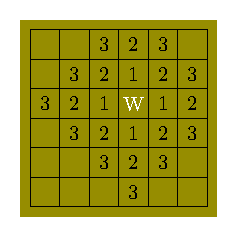
\includegraphics[scale=0.7]{cellular_automata_vision/cellular_automata_vision.pdf}
            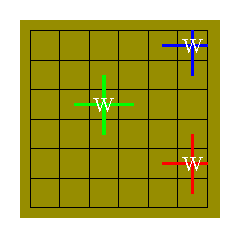
\includegraphics[scale=0.7]{cellular_automata_trueedges/cellular_automata_trueedges.pdf}
        \end{figure}
\end{frame}

\begin{frame}
    \frametitle{Analysis}
\end{frame}

\begin{frame}
    \frametitle{Conclusions and Further Questions}
\end{frame}


\end{document} 






































